\documentclass[a4paper, 12pt, margins=2.5cm]{homework}
\usepackage{tikz}

\usepackage{graphicx}
\usepackage{dsfont}
\usepackage{microtype}
\usepackage{mathrsfs}
\usepackage[ngerman]{babel}
\usepackage{csquotes}
\usepackage[T1]{fontenc}
\usepackage{lmodern}
\usepackage{wasysym}

\setlength{\parindent}{0pt}

\newcommand{\R}{\mathbb{R}}
\newcommand{\N}{\mathbb{N}}
\newcommand{\Z}{\mathbb{Z}}
\newcommand{\Q}{\mathbb{Q}}
\newcommand{\C}{\mathbb{C}}

\name{Tobias Eidelpes}
\course{Objektorientierte Modellierung}
\term{2016SS}
\hwnum{3}
\hwtype{Übungsblatt}
\problemtitle{Aufgabe}
\solutiontitle{Lösung}

\begin{document}

% ERLEDIGT
  \problemnumber{1}
  \begin{problem}
    
  \end{problem}
  \begin{solution} \hfill
    \begin{itemize}
      \item
        \begin{description}
          \item[Sequenzdiagramm] Beschreibt den zeitlichen und logischen
                Nachrichtenfluss.
          \item[Kommunikationsdiagramm] Stellt Beziehungen zwischen Interaktionspartnern
                dar.
          \item[Zeitdiagramm] Drückt Zustandsänderungen der Interaktionspartner aus.
          \item[Interaktionsübersichtsdiagramm] Übersicht über verschiedene Interaktionsdiagramme.
        \end{description}
        Primär zum Modellieren von Nachrichten zwischen verschiedenen Interaktionspartnern
        in bestimmten Kontexten. 

      \item Das Sequenzdiagramm besteht aus der horizontalen Achse, an der die 
            Interaktionspartner angeführt werden und der vertikalen Achse, die 
            die Zeit darstellt.
            Es kann Lebenslinien sowie Nachrichten enthalten.
      
      \item Synchrone Nachrichten sind Nachrichten, bei denen der Sender so lange wartet
            und nichts tut, bis eine Antwort bei ihm angekommen ist. \\
            Asynchrone Nachrichten sind im Prinzip Signale, das heißt der Sender
            sendet seine Nachricht, wartet aber nicht explizit auf eine Antwort, sondern
            erledigt dazwischen zum Beispiel andere Dinge.

      \item Aktive Objekte haben einen eigenen Kontrollfluss, das heißt sie agieren
            unabhängig von anderen Objekten. \\
            Passive Objekte wiederum können beispielsweise von aktiven Objekten
            aufgerufen werden, besitzen aber keinen eigenen Kontrollfluss.
    \end{itemize}
  \end{solution}


% ERLEDIGT
  \problemnumber{2}
  \begin{problem}
    
  \end{problem}
  \begin{solution}\hfill
    \begin{itemize}
      \item Zustandsinvarianten stellen sicher, dass ein bestimmter Zustand zu einem
            bestimmten Zeitpunkt erfüllt ist. \\
            Zeiteinschränkungen können einerseits absolut, andererseits relativ angegeben werden.
            Außerdem gibt es die Möglichkeit nicht nur Zeitpunkte sondern auch Zeitdauern
            zu modellieren.

      \item Für Verzweigungen und Schleifen stehen vier Operatoren zur Verfügung:
            alt, opt, break und loop. \\
            Der \textbf{alt-Operator} entspricht einem if-then-else-Konstrukt. Das heißt
            es wird eine Bedingung beim Operator angegeben und wenn diese wahr ist, 
            dann wird der Inhalt des Operanden ausgeführt. Wenn die Bedingung falsch
            ist, dann wird der Inhalt des else-Operators ausgeführt. Wichtig ist,
            dass hier mehrere Bedingungen angeführt werden können. Nur wenn keine 
            Bedingung wahr ist wird der Inhalt des else-Operators ausgeführt. \\
            Der \textbf{opt-Operator} ist im Prinzip dasselbe wie der alt-Operator, es kann
            aber nur eine Bedingung festgelegt werden. Wenn diese wahr ist, dann 
            wird der Inhalt der Bedingung ausgeführt, wenn nicht, dann läuft die
            Interaktion einfach weiter. Die Bedingung wird dann einfach übersprungen. \\
            Der \textbf{break-Operator} wird ähnlich wie der opt-Operator dargestellt.
            Der Unterschied ist der, dass der break Operator, wenn die Bedingung
            wahr ist, den Inhalt der Bedingung ausführt und dann aber nichts mehr
            ausführt und jegliche Interaktionen die danach kommen überspringt. \\
            Der \textbf{loop-Operator} führt bestimmte Interaktionen so lange aus, 
            bis die anfängliche Bedingung nicht mehr wahr ist. 

      \item Für parallele Abläufe und Ordnungen stehen vier Operatoren zur Verfügung:
            seq, strict, par, critical. \\
            Der \textbf{seq-Operator} stellt die Default-Ordnung dar. Hier können
            aber die einzelnen Nachrichten vertauscht werden, wenn es die Interaktionspartner
            zulassen. \\
            Der \textbf{strict-Operator} legt fest, in welcher Reihenfolge die Nachrichten
            ausgetauscht werden müssen. Hier kann man die Reihenfolge auf keinen
            Fall verändern. \\
            Der \textbf{par-Operator} ermöglicht es Nachrichten in irgendeiner
            Reihenfolge zu verschicken, solange die Nachrichten auf der lokalen
            Zeitachse der Interaktionspartner der durch den seq-Operator festgelegten
            Reihenfolge folgen. \\
            Der \textbf{critical-Operator} legt eine Menge an Nachrichten fest,
            die in der festgelegten Reihenfolge ablaufen müssen und nicht unterbrochen
            werden dürfen. 

      \item Für Filterungen und Zusicherungen gibt es folgende Operatoren:
            ignore, consider, assert, neg. \\
            Der \textbf{ignore-Operator} gibt Nachrichten an, die auftreten
            aber getrost ignoriert werden können. \\
            Der \textbf{consider-Operator} ist das Gegenstück zum ignore-Operator
            und wird verwendet um Nachrichten hervorzuheben. \\
            Der \textbf{assert-Operator} besagt, dass Nachrichten genau so ausgeführt
            werden sollen und es keine Abweichungen geben darf. \\
            Der \textbf{neg-Operator} drückt einen Sachverhalt aus, der nicht 
            eintreten darf. 
    \end{itemize}
  \end{solution}


% ERLEDIGT
  \problemnumber{3}
  \begin{problem}
    
  \end{problem}
  \begin{solution}\hfill
    \begin{center}
      \def\svgwidth{1\textwidth}\input{Aufgabe3.pdf_tex}  
    \end{center}
  \end{solution}


% ERLEDIGT
  \problemnumber{4}
  \begin{problem}
    
  \end{problem}
  \begin{solution} \hfill
    \begin{enumerate}[label=\alph*)]\itemsep0pt
      \item
        \begin{itemize}  
          \item Die beiden Diagramme sind \textbf{nicht äquivalent}, weil bei a) die
                Nachricht b auf jeden Fall verschickt wird und bei b) nur dann, wenn
                \texttt{x != 5} ist.

          \item Die beiden Diagramme sind \textbf{äquivalent}.

          \item Die beiden Diagramme sind \textbf{äquivalent}.
        \end{itemize}

      \item 
        \begin{itemize}
          \item In strict muss genau diese Reihenfolge eingehalten werden: $b\rightarrow c$.
          \item Im par-Teil ist die Reihenfolge irrelevant, außer dass g nach d
                kommen muss und e und f direkt aufeinanderfolgend sein müssen und
                e nach d und vor g stehen muss.
                \[ d\rightarrow e\rightarrow f\rightarrow g\rightarrow h \]
                \[ h\rightarrow d\rightarrow e\rightarrow f\rightarrow g  \]
        \end{itemize}
    \end{enumerate}
  \end{solution}


% AUSSTÄNDIG
  \problemnumber{5}
  \begin{problem}
    
  \end{problem}
  \begin{solution}\hfill
    \begin{center}
      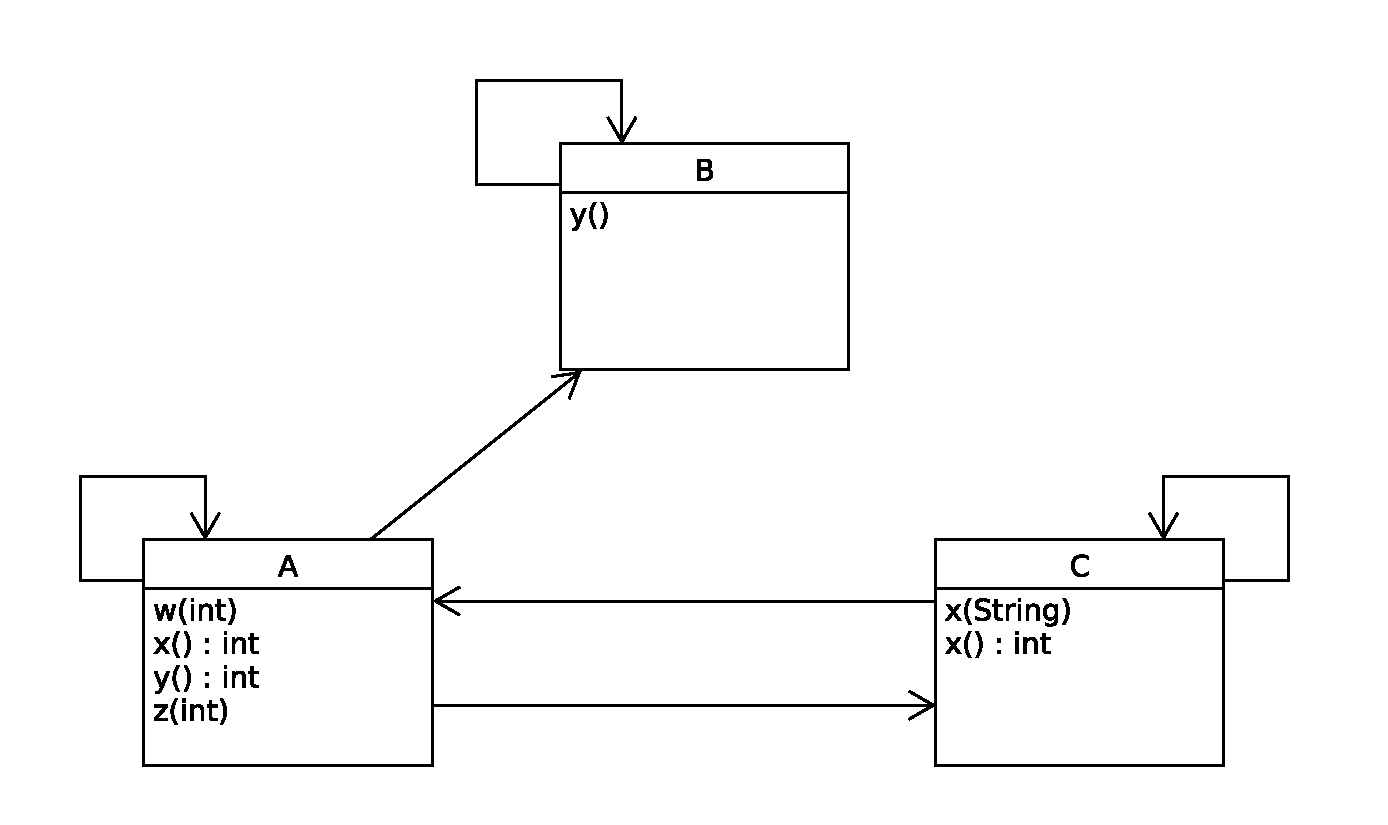
\includegraphics[scale=0.6]{Aufgabe5.eps}
    \end{center}
  \end{solution}


% AUSSTÄNDIG
  \problemnumber{6}
  \begin{problem}
    
  \end{problem}
  \begin{solution}
    
  \end{solution}

\end{document}